\documentclass[tikz,border=10pt]{standalone}
\usepackage{tikz}
\usetikzlibrary{shapes.geometric, arrows, arrows.meta, positioning, fit, backgrounds, decorations.pathreplacing, calc}

\begin{document}
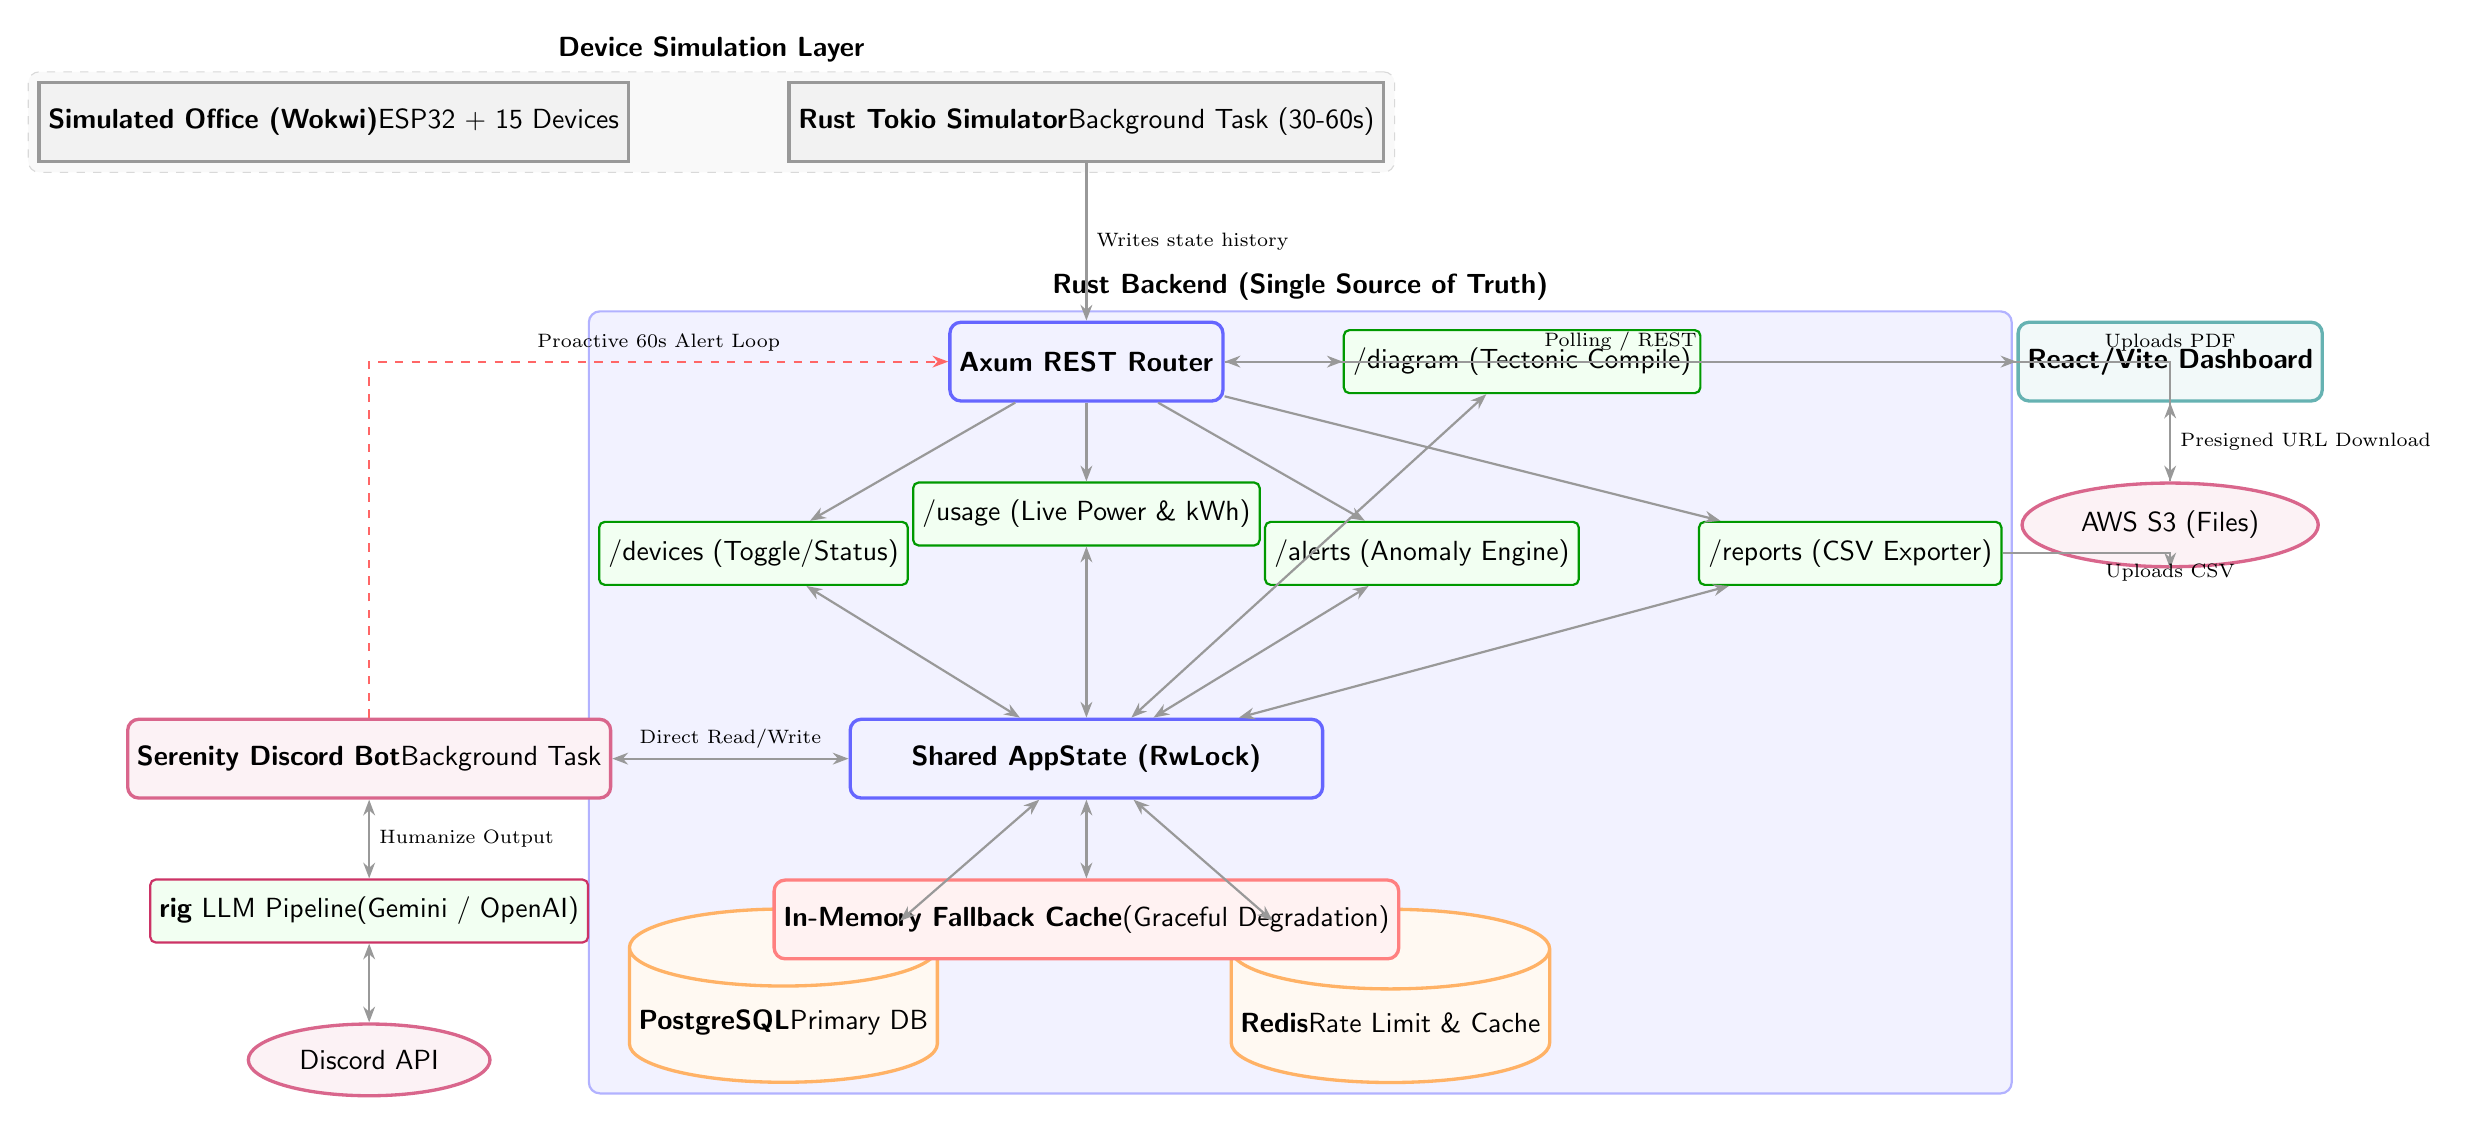
\begin{tikzpicture}[
    node distance=1.5cm and 2cm,
    font=\sffamily,
    % Core Shapes
    rect/.style={rectangle, draw=blue!60, fill=blue!5, very thick, minimum width=3cm, minimum height=1cm, text centered, rounded corners},
    db/.style={cylinder, shape border rotate=90, aspect=0.25, draw=orange!60, fill=orange!5, very thick, minimum width=2.2cm, minimum height=2.2cm, text centered},
    api_node/.style={rectangle, draw=green!60!black, fill=green!5, thick, minimum width=2.5cm, minimum height=0.8cm, text centered, rounded corners=2pt},
    external/.style={ellipse, draw=purple!60, fill=purple!5, very thick, text centered, inner sep=0.2cm},
    hw/.style={rectangle, draw=gray!80, fill=gray!10, very thick, minimum width=3cm, minimum height=1cm, text centered},
    % Connectors
    line/.style={thick, draw=gray!80, -{Stealth[length=2mm]}},
    bidir/.style={thick, draw=gray!80, {Stealth[length=2mm]}-{Stealth[length=2mm]}},
    dashed_line/.style={thick, dashed, draw=red!60, -{Stealth[length=2mm]}},
]

% 1. Simulated Hardware Layer
\node[hw] (esp) {\textbf{Simulated Office (Wokwi)}\\ESP32 + 15 Devices};
\node[hw, right=of esp] (sim) {\textbf{Rust Tokio Simulator}\\Background Task (30-60s)};

\begin{scope}[on background layer]
    \node[fill=gray!5, draw=gray!30, dashed, fit=(esp)(sim), rounded corners, label=above:\textbf{Device Simulation Layer}] (sim_layer) {};
\end{scope}

% 2. Backend Core (Axum)
\node[rect, below=2cm of sim] (axum) {\textbf{Axum REST Router}};

% Controllers
\node[api_node, below left=1.5cm and 0.5cm of axum] (devices) {/devices (Toggle/Status)};
\node[api_node, below=1cm of axum] (usage) {/usage (Live Power \& kWh)};
\node[api_node, below right=1.5cm and 0.5cm of axum] (alerts) {/alerts (Anomaly Engine)};
\node[api_node, right=1.5cm of axum] (diagram) {/diagram (Tectonic Compile)};
\node[api_node, right=1.5cm of alerts] (reports) {/reports (CSV Exporter)};

% Shared State & DB
\node[rect, below=4cm of axum, minimum width=6cm] (state) {\textbf{Shared AppState (RwLock)}};
\node[db, below left=1.5cm and -0.5cm of state] (pg) {\textbf{PostgreSQL}\\Primary DB};
\node[db, below right=1.5cm and -0.5cm of state] (redis) {\textbf{Redis}\\Rate Limit \& Cache};
\node[rect, draw=red!50, fill=red!5, below=1cm of state] (mem) {\textbf{In-Memory Fallback Cache}\\(Graceful Degradation)};

\begin{scope}[on background layer]
    \node[fill=blue!5, draw=blue!30, thick, fit=(axum)(devices)(usage)(alerts)(diagram)(reports)(state)(mem)(pg)(redis), rounded corners, label=above:\textbf{Rust Backend (Single Source of Truth)}] (backend_layer) {};
\end{scope}

% 3. Discord Bot
\node[rect, draw=purple!60, fill=purple!5, left=3cm of state] (bot) {\textbf{Serenity Discord Bot}\\Background Task};
\node[api_node, draw=purple!80, below=1cm of bot] (llm) {\textbf{rig} LLM Pipeline\\(Gemini / OpenAI)};
\node[external, below=1cm of llm] (discord) {Discord API};

% 4. Web Dashboard
\node[rect, draw=teal!60, fill=teal!5, right=4cm of diagram] (web) {\textbf{React/Vite Dashboard}};
\node[external, below=1cm of web] (s3) {AWS S3 (Files)};

% Connections
% Sim to DB
\draw[line] (sim) -- node[right, font=\scriptsize] {Writes state history} (axum);

% Axum to Controllers
\draw[line] (axum) -- (devices);
\draw[line] (axum) -- (usage);
\draw[line] (axum) -- (alerts);
\draw[line] (axum) -- (diagram);
\draw[line] (axum) -- (reports);

% Controllers to State
\draw[bidir] (devices) -- (state);
\draw[bidir] (usage) -- (state);
\draw[bidir] (alerts) -- (state);
\draw[bidir] (diagram) -- (state);
\draw[bidir] (reports) -- (state);

% State to DBs
\draw[bidir] (state) -- (pg);
\draw[bidir] (state) -- (redis);
\draw[bidir] (state) -- (mem);

% Bot Connections
\draw[bidir] (bot) -- node[above, font=\scriptsize] {Direct Read/Write} (state);
\draw[bidir] (bot) -- node[right, font=\scriptsize] {Humanize Output} (llm);
\draw[bidir] (llm) -- (discord);
\draw[dashed_line] (bot) |- node[near end, above, font=\scriptsize] {Proactive 60s Alert Loop} (axum);

% Web Connections
\draw[bidir] (web) -- node[above, font=\scriptsize] {Polling / REST} (axum);
\draw[line] (diagram) -| node[above, font=\scriptsize] {Uploads PDF} (s3);
\draw[line] (reports) -| node[below, font=\scriptsize] {Uploads CSV} (s3);
\draw[line] (s3) -- node[right, font=\scriptsize] {Presigned URL Download} (web);

\end{tikzpicture}
\end{document}
